\chapter{Realizace projektu Importér}
\label{chap:importer_implementation}

Tato kapitola popisuje technickou realizaci klíčové části odborné praxe – modulu Importér. Řešení je rozděleno do tří vrstev: databázové, aplikační (backend) a prezentační (frontend).

\section{Analýza a návrh databáze}

Databázová vrstva je implementována na platformě Microsoft SQL Server \cite{sqlserver_docs} pod vyhrazeným schématem \texttt{importer}. Architektura byla navržena s důrazem na konfigurovatelnost, což umožňuje definovat nové typy importů bez nutnosti zásahů do zkompilovaného kódu aplikace.

Model dat se skládá ze tří logických celků:
\begin{enumerate}
    \item \textbf{Definice struktury:} Metadata popisující, jaká data lze importovat (kontexty, sloupce).
    \item \textbf{Konfigurace šablon:} Uložení uživatelských nastavení a mapování.
    \item \textbf{Provozní data:} Logování průběhu importu a auditní stopy.
\end{enumerate}

\subsection{Klíčové entity a vztahy}

Základním stavebním kamenem je tabulka \texttt{CTypy}, která slouží jako kořenový číselník pro logickou separaci dat. Na ni navazuje hierarchická struktura definovaná v tabulce \texttt{Kontext}. Významným prvkem návrhu je rekurzivní vazba v tabulce \texttt{Kontext} přes sloupec \texttt{IdKontextNadrizeny}, což umožňuje modelovat vnořené objekty (např. Subjekt $\rightarrow$ Adresa $\rightarrow$ Kontakt).

\begin{figure}[h]
    \centering
    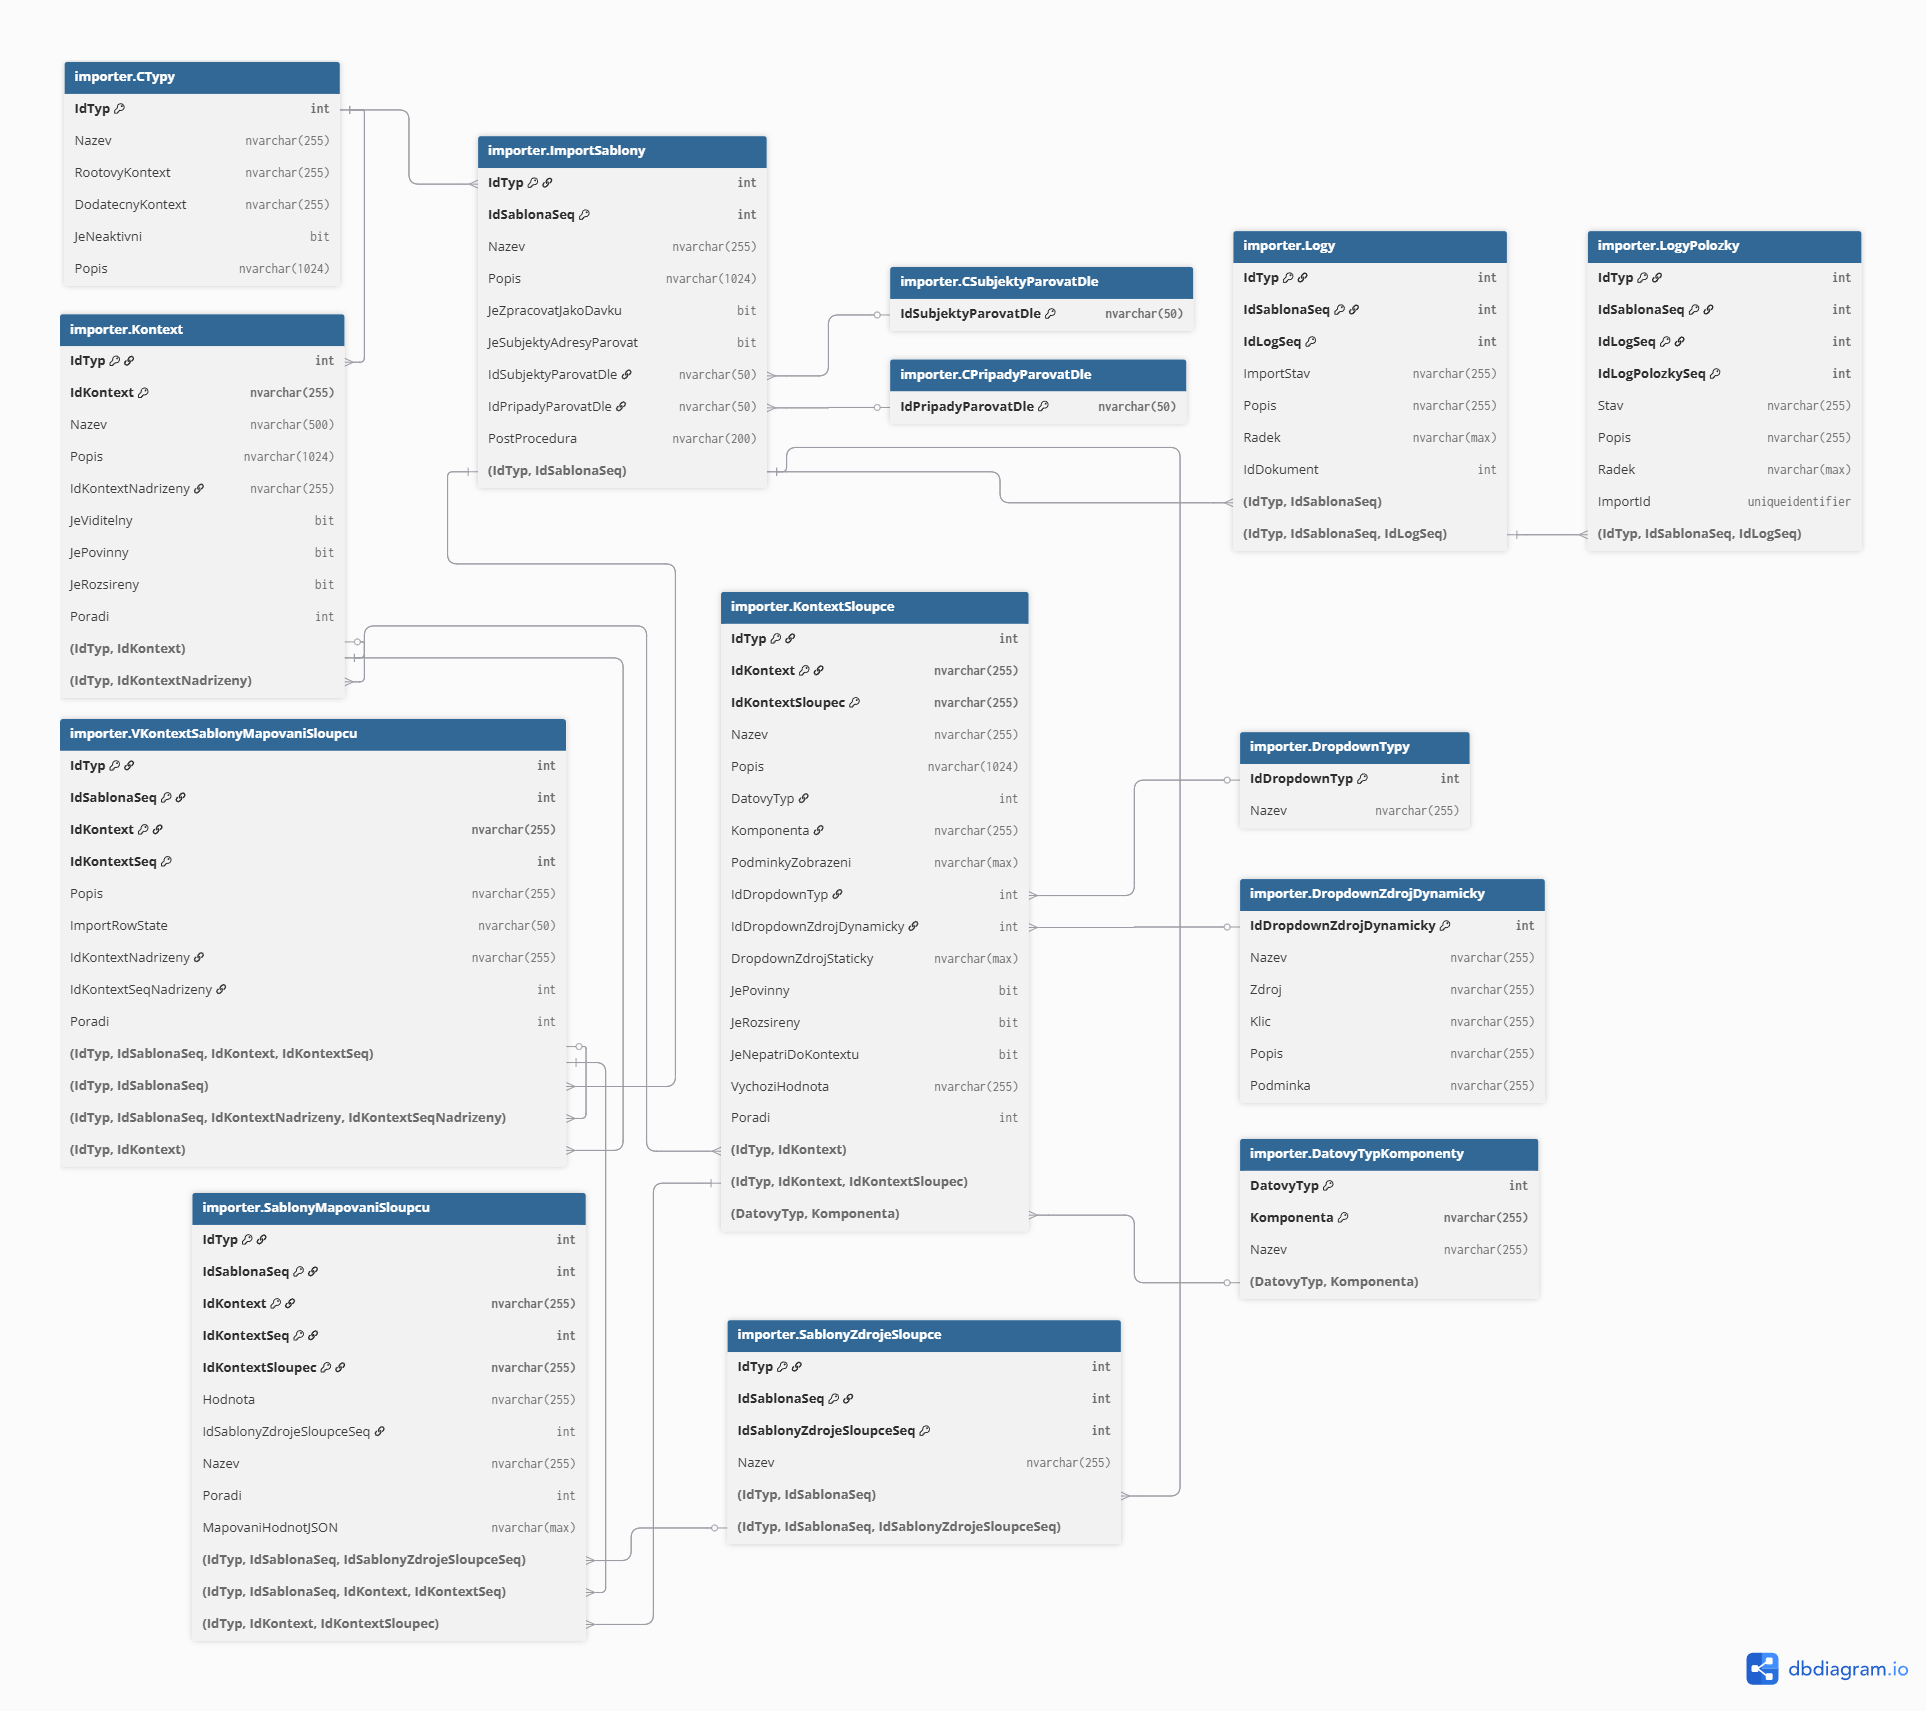
\includegraphics[width=0.8\textwidth]{Figures/ERD_Importer.png}
    \caption{Zjednodušený ER diagram databázového schématu Importer}
    \label{fig:erd_diagram}
\end{figure}

\section{Serverová část a aplikační logika}

Backendová část řešení je implementována v jazyce C\# \cite{csharp_docs} jako \textbf{Service Fabric Actor} v rámci platformy EFabric. Jedná se o mikroslužbu běžící v prostředí Microsoft Azure \cite{microsoft_servicefabric}.

Propojení s jádrem systému zajišťuje třída \texttt{ImporterContext}, která dědí z \texttt{EMapContext}. Samotný proces importu probíhá asynchronně ve dvou fázích: nejprve validace a příprava dat (\texttt{CreateImportAsync}) a následně fyzický zápis do cílových tabulek (\texttt{DirectImportAsync}).

\section{Uživatelské rozhraní (Frontend)}

Prezentační vrstva modulu Importér představuje nejrozsáhlejší část realizace. Je navržena jako autonomní feature modul (\texttt{ImporterModule}) v rámci enterprise architektury systému Evolio, využívající verzi \textbf{Angular 17} \cite{angular_docs} a \textbf{TypeScript} \cite{typescript_docs}.

\subsection{Architektura a hierarchie komponent}

Modul je dekomponován na osm specializovaných komponent, které spolupracují na zajištění plynulého uživatelského zážitku při zpracování dat. Využití komponentového přístupu umožňuje oddělit logiku zobrazení od orchestrace dat. Detailní přehled všech komponent uvádí tabulka \ref{tab:fe_components_full}.



\begin{table}[h]
\centering
\caption{Kompletní přehled komponent modulu Importér}
\label{tab:fe_components_full}
\begin{tabular}{|l|p{9cm}|}
\hline
\textbf{Komponenta} & \textbf{Účel a hlavní funkce} \\ \hline
\texttt{ImporterDetailComponent} & Hlavní dashboard. Zobrazuje typy importů, historii logů a náhled dat ze souboru. \\ \hline
\texttt{ImporterMappingComponent} & Klíčová obrazovka pro definici mapování sloupců Excelu na kontexty systému. \\ \hline
\texttt{ContextTreeComponent} & Rekurzivní komponenta pro vizualizaci a navigaci v hierarchickém stromu kontextů. \\ \hline
\texttt{ImporterDropdownComponent} & Specializovaný výběrový prvek pro intuitivní přiřazování sloupců k atributům. \\ \hline
\texttt{ValueMappingModalComponent} & Dialog pro definici transformací hodnot (např. převod textových stavů na číselné ID). \\ \hline
\texttt{DocumentPickerButtonComponent} & Prvek pro nahrávání souborů s podporou validace přípon a velikosti. \\ \hline
\texttt{ImportProgressDialogComponent} & Sleduje průběh importu po řádcích v reálném čase s vizualizací úspěšnosti. \\ \hline
\texttt{ImportLogDetailComponent} & Detailní prohlížeč výsledků a chybových zpráv z proběhlých importů. \\ \hline
\end{tabular}
\end{table}

\begin{figure}[H]
    \centering
    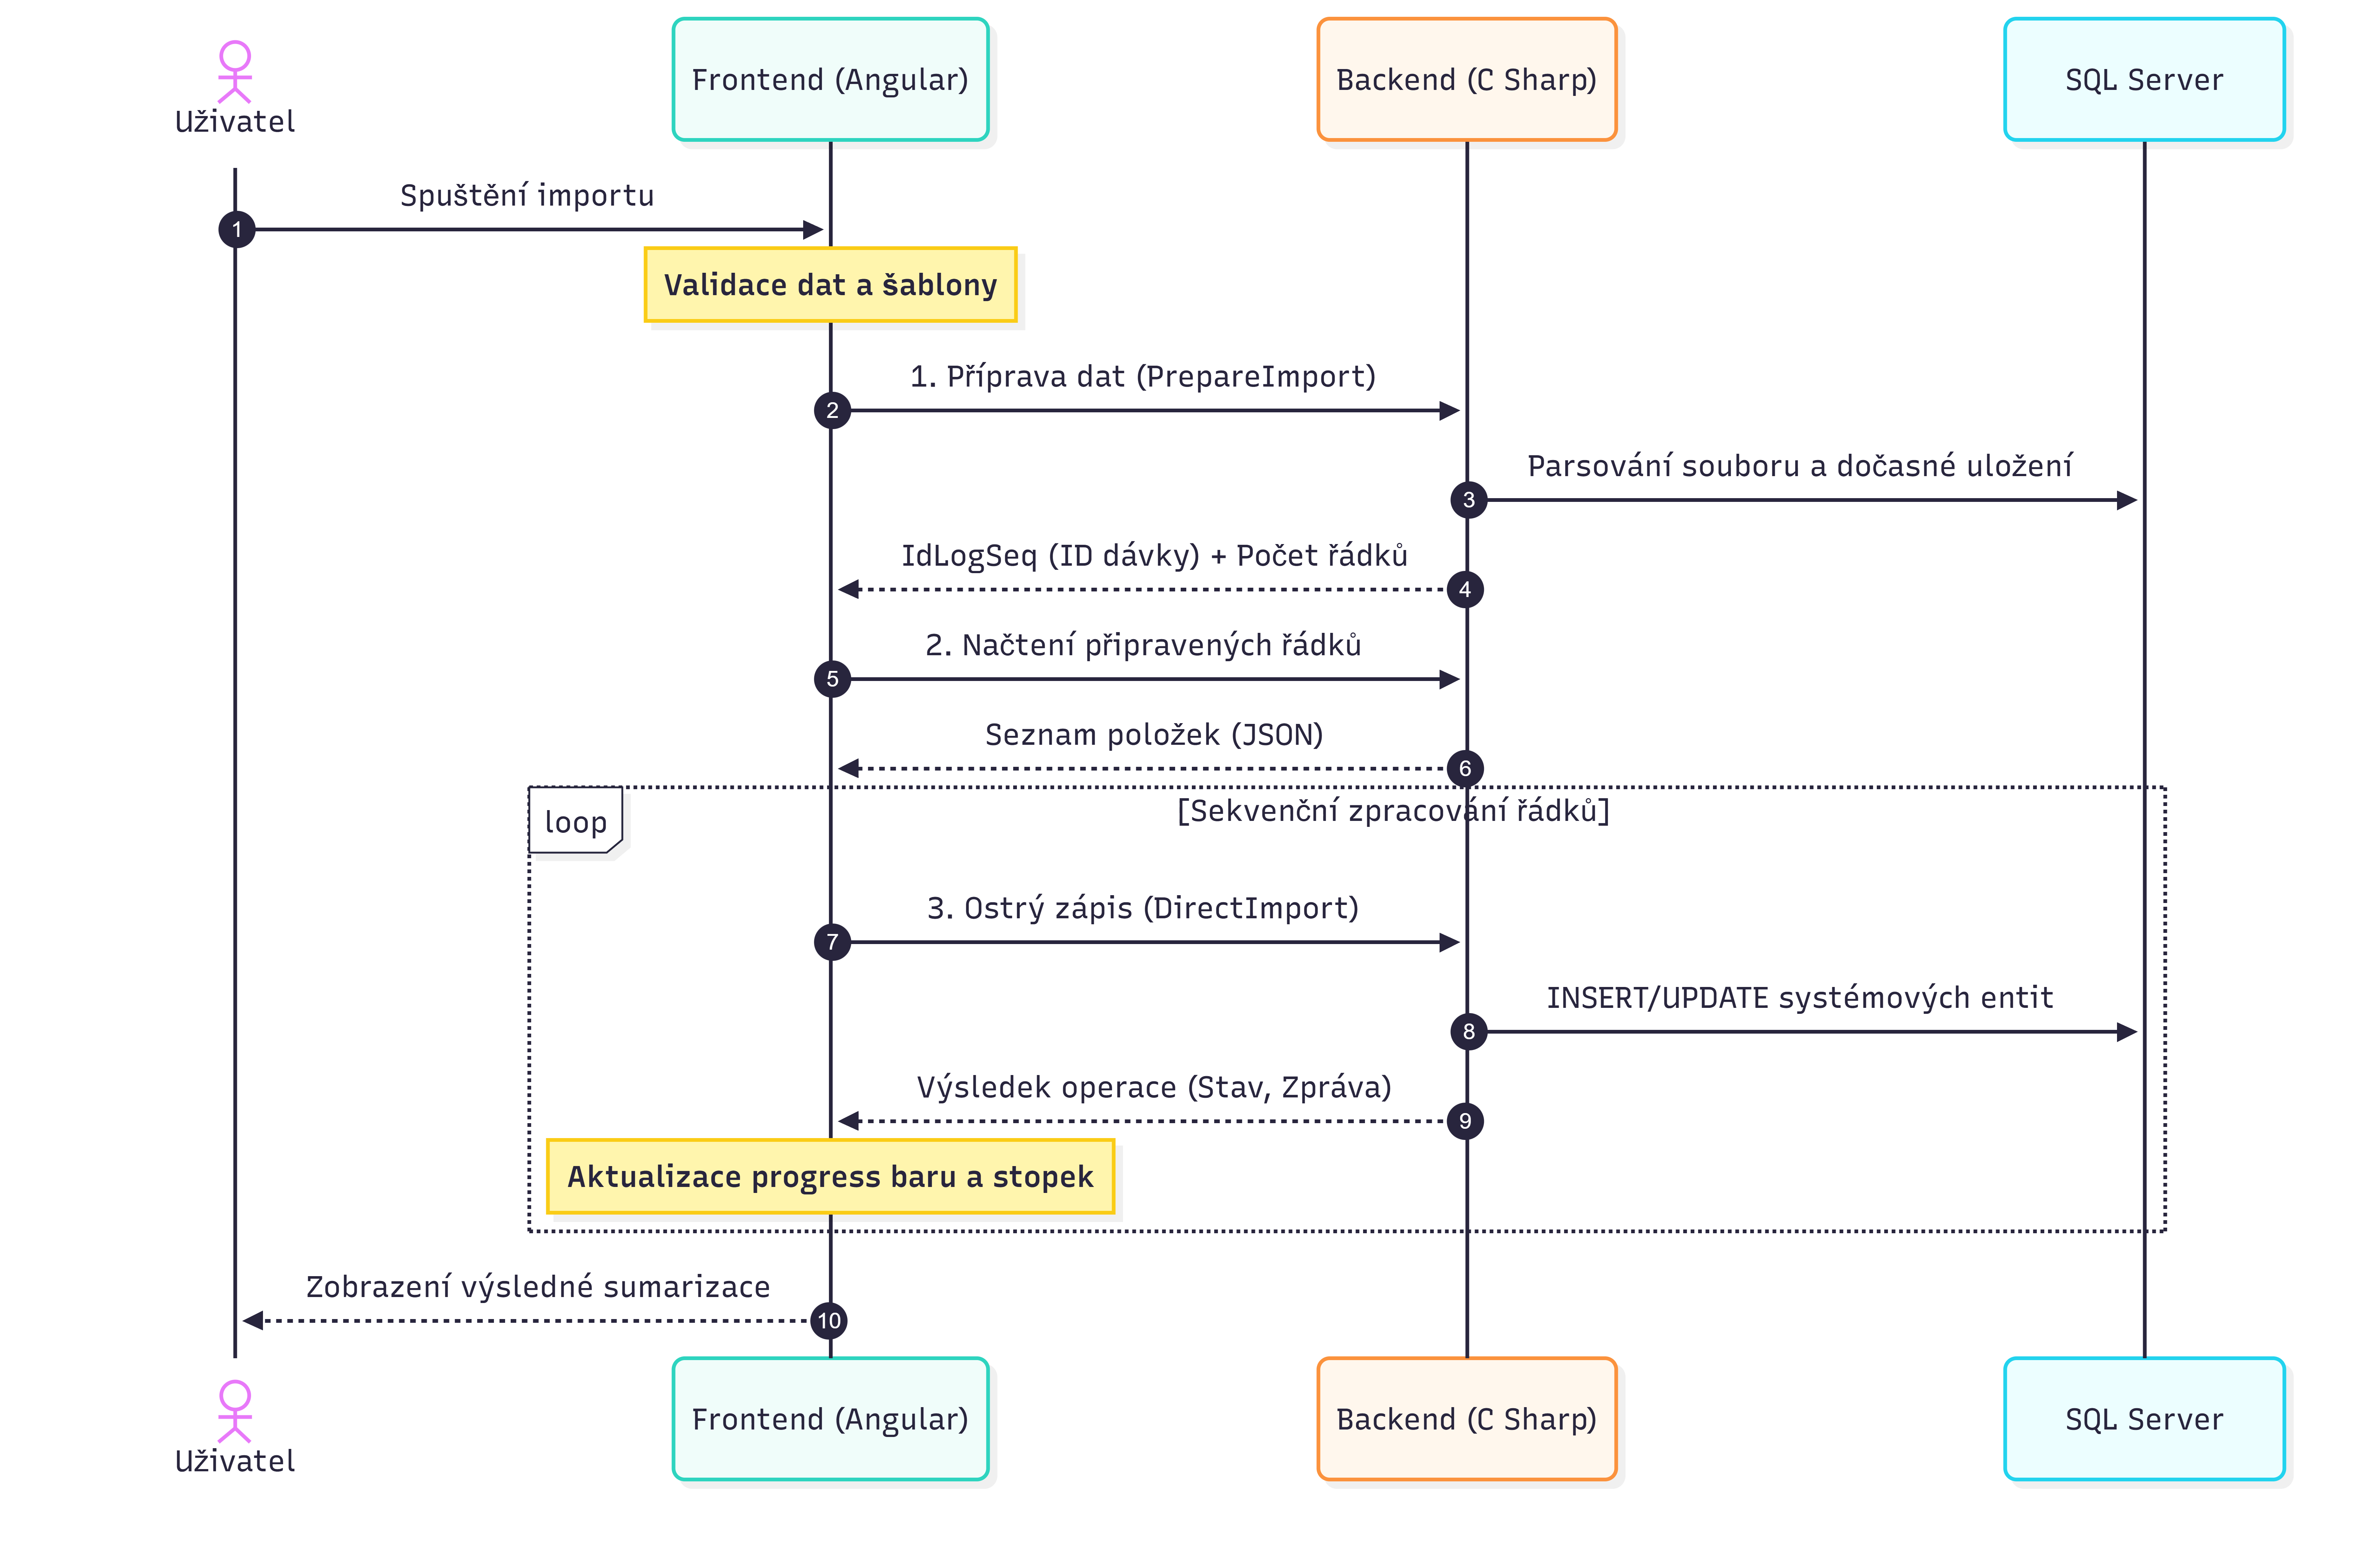
\includegraphics[width=1\textwidth]{Figures/diagram.png}
    \caption{Sekvenční diagram procesu zpracování importu po jednotlivých řádcích}
    \label{fig:import_sequence}
\end{figure}

\subsection{Moderní reaktivní vzory: Signály a RxJS}

Aplikace využívá kombinaci tradiční knihovny RxJS \cite{rxjs_docs} a nového reaktivního primitiva \textbf{Signals}, představeného v Angularu 17. Signály jsou použity pro správu synchronního stavu, který nevyžaduje komplexní transformace, což zjednodušuje kód a zvyšuje čitelnost.

V rámci \texttt{ImporterService} jsou signály využity pro sledování aktuálního kontextu:
\begin{lstlisting}[language=Java, caption={Využití signálů pro správu stavu modulu}]
// Definice signálu pro sledování vybrané šablony
public selectedSablonaId = signal<number | null>(null);

// Výpočetní signál závislý na změně ID
public isSablonaSelected = computed(() => this.selectedSablonaId() !== null);
\end{lstlisting}

Pro asynchronní operace, jako je paralelní načítání číselníků při inicializaci, je nadále využíváno RxJS. Operátor \texttt{forkJoin} zajišťuje, že se aplikace vykreslí až v momentě, kdy jsou k dispozici všechna potřebná metadata:

\begin{lstlisting}[language=Java, caption={Paralelní inicializace dat pomocí forkJoin}]
forkJoin({
  typy: this.emap.get('cTypy', { IdTyp: this.idTyp() }),
  kontexty: this.emap.get('kontext', { IdTyp: this.idTyp() }),
  sablony: this.emap.get('importSablony', { IdTyp: this.idTyp() })
}).pipe(takeUntil(this.destroy$)).subscribe(data => {
  this.state.update(s => ({ ...s, ...data }));
});
\end{lstlisting}

\subsection{Optimalizace výkonu pomocí OnPush strategie}

Z důvodu vysokých nároků na výkon při zobrazování rozsáhlých mapovacích struktur (stromy s desítkami uzlů) byla u všech komponent nasazena strategie \textbf{ChangeDetectionStrategy.OnPush}. 

Tato optimalizace instruuje Angular, aby kontčistých rouroloval změny v komponentě pouze v případě, že se změní její vstupní reference (\texttt{@Input}) nebo je změna explicitně vyžádána. Tím se výrazně redukuje počet cyklů detekce změn při interakci uživatele s formulářem.

\begin{lstlisting}[language=Java, caption={Definice komponenty s OnPush strategií}]
@Component({
  selector: 'ev-importer-mapping',
  templateUrl: './importer-mapping.component.html',
  styleUrls: ['./importer-mapping.component.scss'],
  changeDetection: ChangeDetectionStrategy.OnPush
})
export class ImporterMappingComponent { ... }
\end{lstlisting}

\subsection{Implementace komplexní mapovací logiky}

Jádrem modulu je \texttt{ImporterMappingComponent}, která umožňuje uživateli interaktivně sestavit strukturu importu. Na rozdíl od původního desktopového řešení se zde uplatňuje princip \textit{on-demand} budování struktury:

\begin{itemize}
    \item \textbf{Dynamické instance:} Uživatel může přidávat více instancí stejného kontextu (např. více adres k jednomu subjektu). Každá instance má vlastní stav mapování sloupců.
    \item \textbf{Interaktivní správa:} Stav sbalení a rozbalení jednotlivých sekcí je udržován v \texttt{Set<string>}, což zajišťuje rychlou manipulaci i při velkém počtu prvků.
    \item \textbf{Datová transformace:} Pomocí \textit{pure pipes} dochází k transformaci dat bez nutnosti přepočítávání při každém cyklu detekce změn.
\end{itemize}

\subsection{Real-time monitoring a UX prvky}

Proces importu probíhá sekvenčně, přičemž uživatel je o postupu informován prostřednictvím \texttt{ImportProgressDialogComponent}. Tato komponenta kombinuje několik technologií pro zajištění plynulé zpětné vazby:

\begin{itemize}
    \item \textbf{Sledování času:} Využití knihovny \textit{moment.js} v sekundovém intervalu pro zobrazení doby trvání importu.
    \item \textbf{Inkrementální DataGrid:} Výsledky jsou do tabulky (\textit{DevExtreme DataGrid}) přidávány okamžitě po dokončení požadavku na konkrétní řádek.
    \item \textbf{Vizuální indikátory:} Namísto statických spinnerů jsou v dashboardu využity \textbf{skeleton loadingy}, které predikují strukturu obsahu a snižují kognitivní zátěž uživatele při čekání na data.
\end{itemize}